%%%%%%%%%%%%%%%%%%%%%%%%%%%%%%%%%%%%%%
\section{Results} \label{results}
%%%%%%%%%%%%%%%%%%%%%%%%%%%%%%%%%%%%%%
% \begin{figure}
%     \centering
%     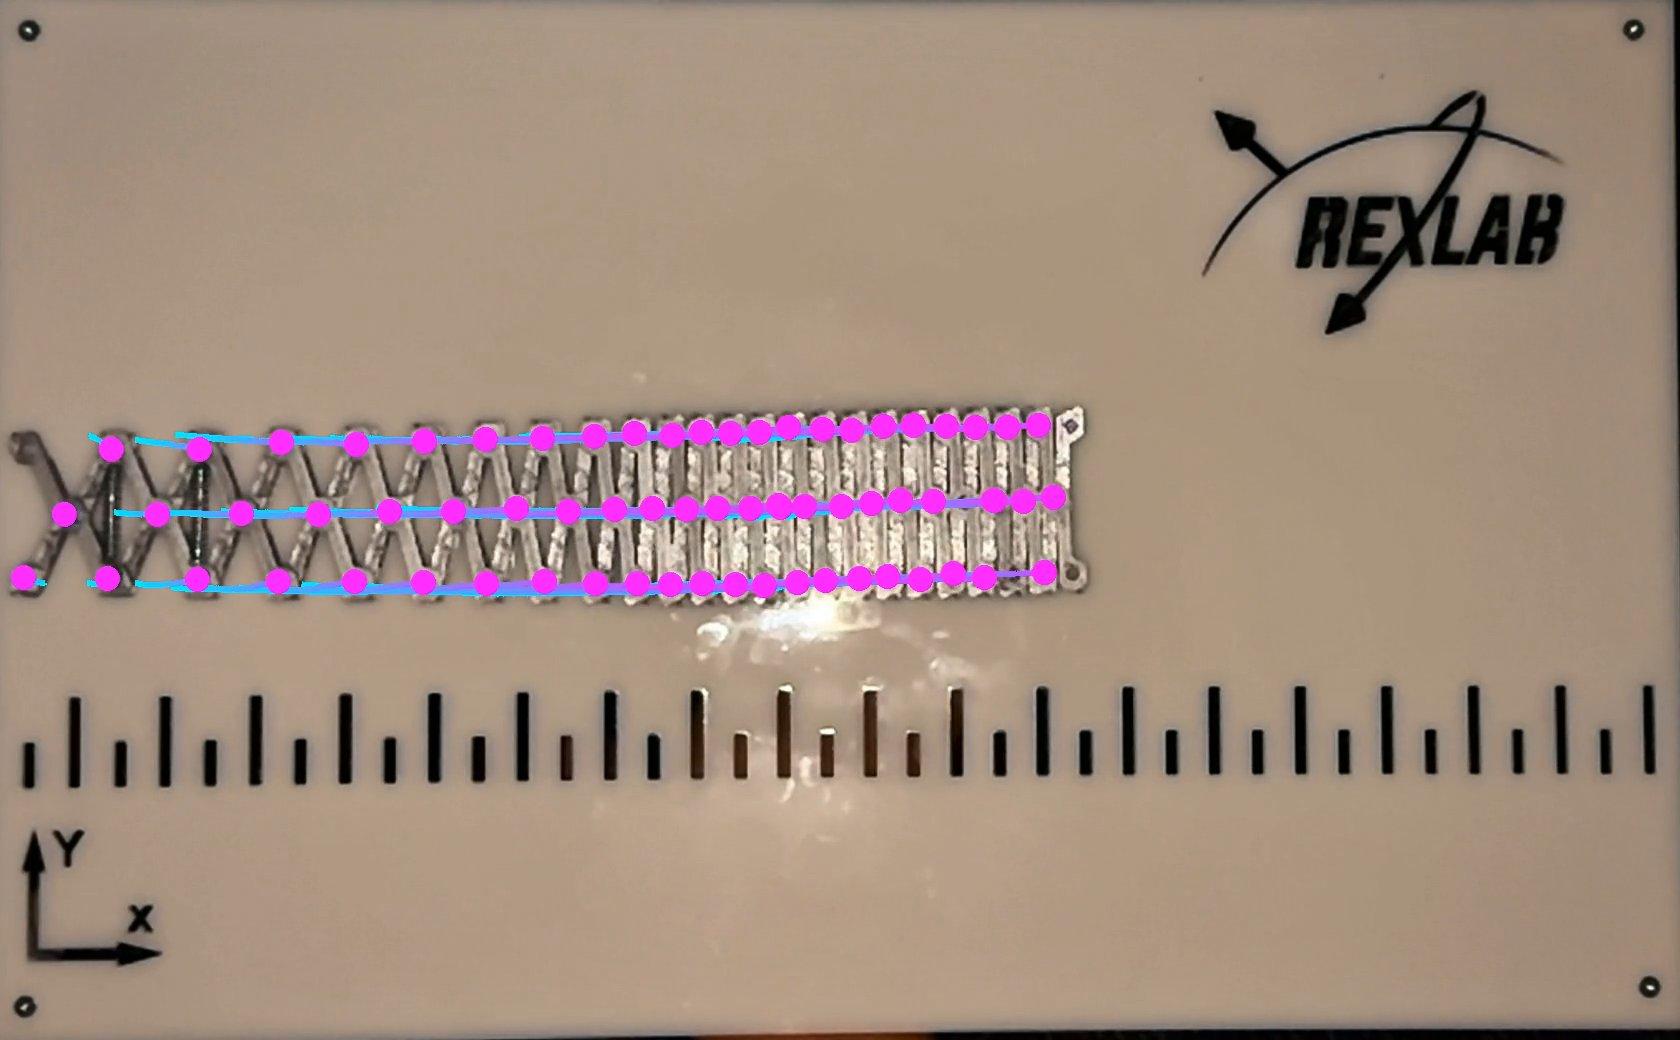
\includegraphics[width=\linewidth]{DOJO-CCK/Figures/Image_scissor_tracking.png}
%     \caption{Caption}
%     \label{fig:enter-label}
% \end{figure}
\begin{figure}
    \centering
    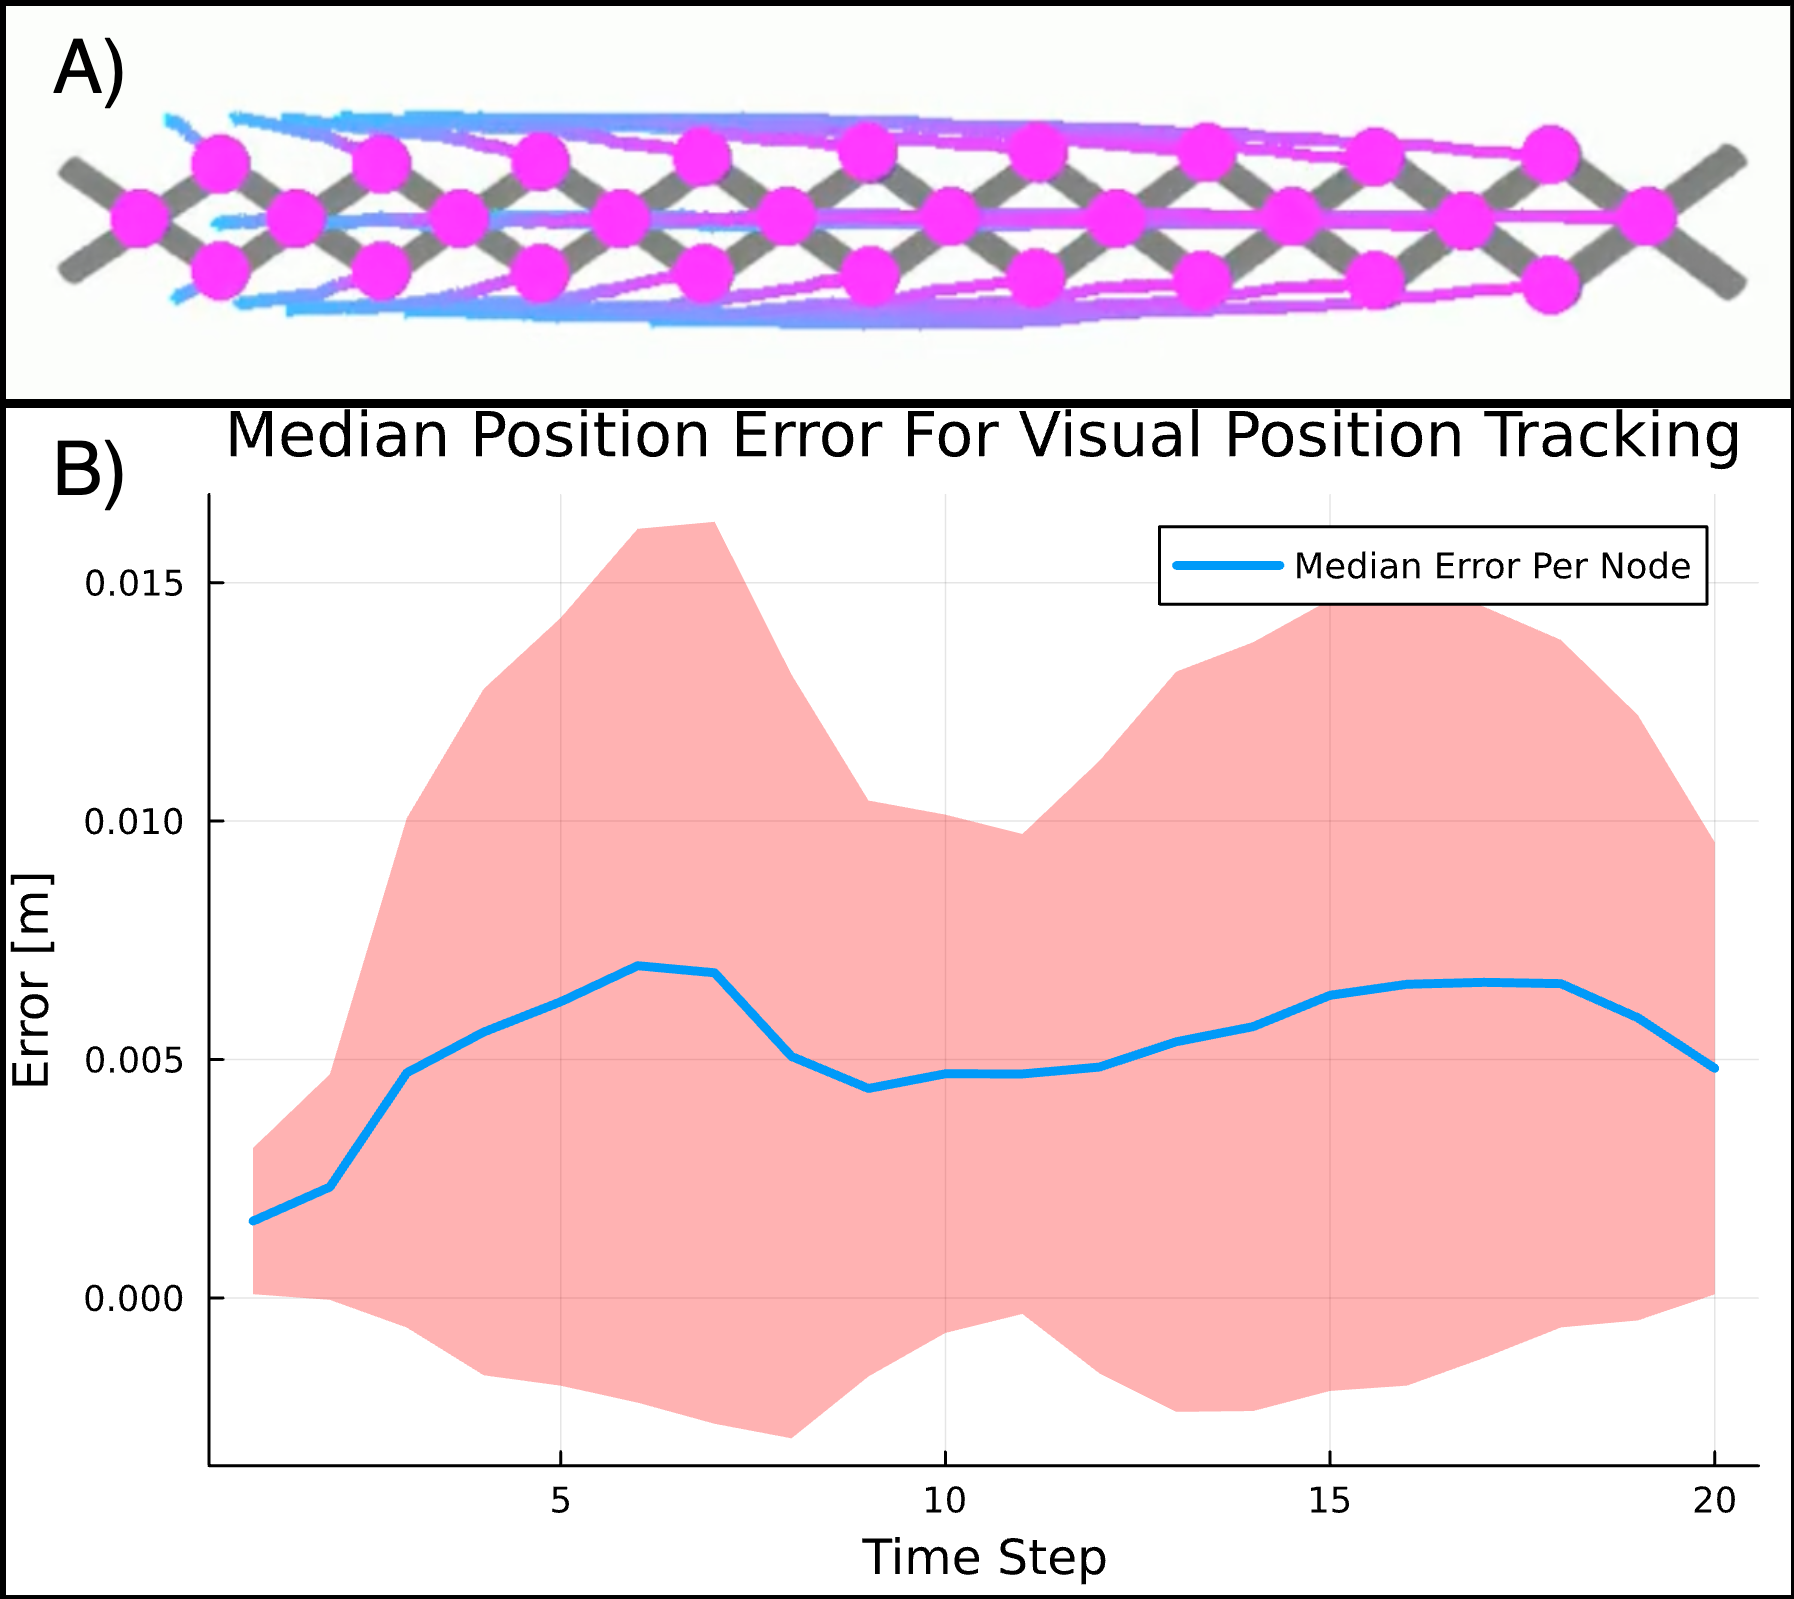
\includegraphics[width=\linewidth]{Figures/tracking_error.drawio.png}
    \caption{ (A) Visual tracking result of the co-tracker on the synthetic scissor mechanism, with tracked points indicated in pink and position history tails. (B) Median position error for visual tracking from ground truth synthetic data per node per time step. The blue line represents the median error per node across each time step, and the shaded red region indicates the range of error variation using median absolute error.}
    \label{fig:sim_to_sim-tracking}
    
\end{figure}
\begin{figure}
    \centering
    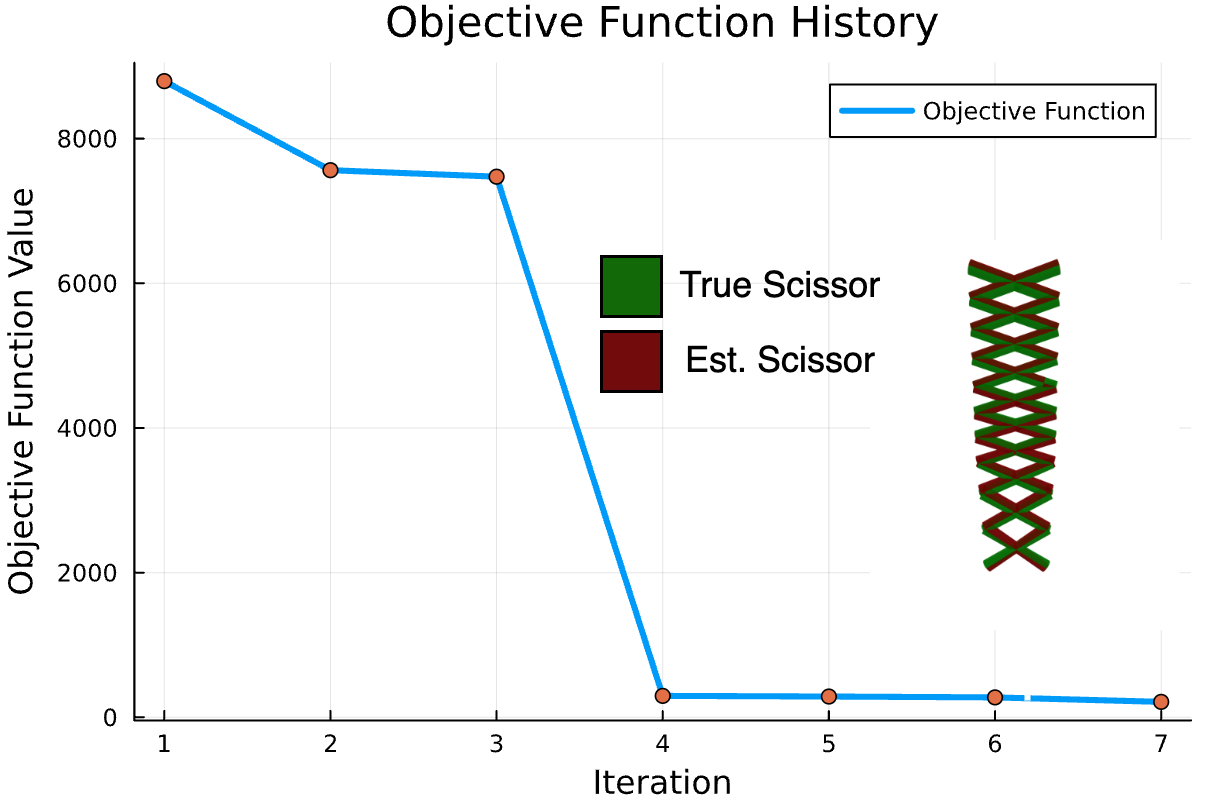
\includegraphics[width=\linewidth]{Figures/simulation_to_simulation_sys_id.drawio.png}
    \caption{Objective function history from LBFGS algorithm for joint clearance and friction estimation, comparing synthetic data with estimated data. The plot shows the objective function value decreasing over iterations as the estimated scissor mechanism (in red) converges to match the true scissor mechanism (in green).}
    \label{fig:sim_to_sim-LBFGS}
\end{figure}
\begin{figure}
    \centering
    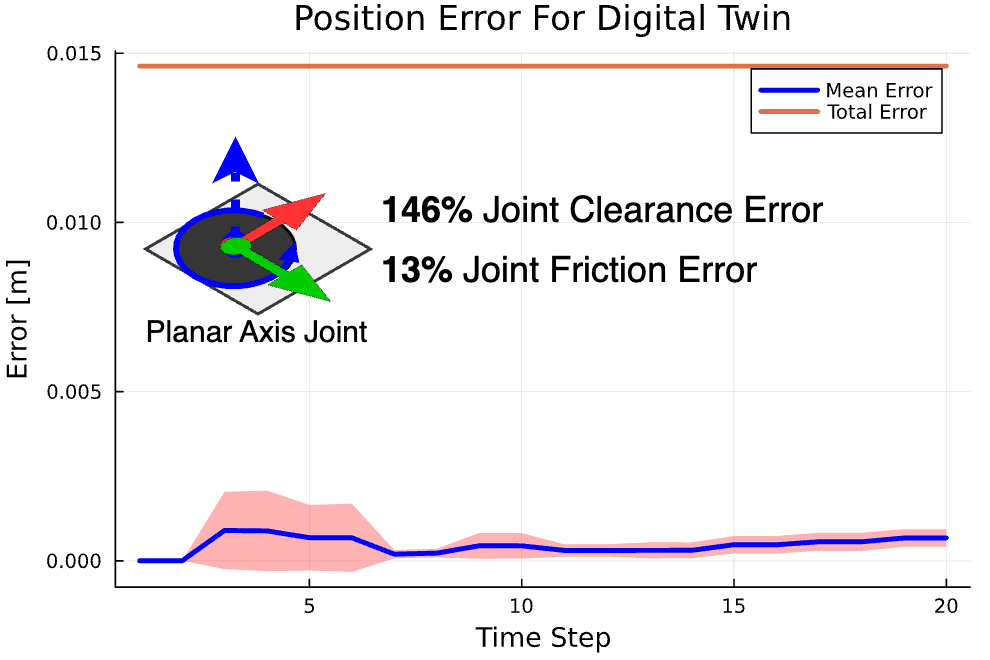
\includegraphics[width=\linewidth]{Figures/simulation_to_simulation_error.drawio.png}
    \caption{Position error for the digital twin, showing the mean error (blue line) and total error (red line) over all time steps. The solution had a 146\% joint clearance error and a 13\% joint friction error. The shaded region represents the variability in position error across time.}
    \label{fig:sim_to_sim-Error}
\end{figure}
\subsection{Synthetic Data results results}
\subsubsection{Visual Analysis}
We evaluate the co-motion optical tracking program using synthetic data generated by our physics engine. The co-motion model was given a pixel mask where joint locations were in the last frame, and the system returned the positions for all video frames. The result of the synthetic data tracking can be seen in Figure \ref{fig:sim_to_sim-tracking} A. These results were then compared with the true joint locations, and the median position error over 20 timesteps is shown in Figure \ref{fig:sim_to_sim-tracking} B. The per-node frame error had a median value of around 5 millimeters. Given that the joint slop to generate the synthetic data was around 1 millimeter, this visual tracking does not provide an ideal resolution for this particular application. Higher-resolution state estimation methods like fiducial markers will be explored in future work. 

\subsubsection{System Identification}
Next, we evaluated the joint optimization from \eqref{eq:optim} using idealized data generated from the physics engine. Equation \eqref{eq:optim} is solved using the LBFGS algorithm. The convergence of the parameters is shown in Figure \ref{fig:sim_to_sim-LBFGS}, and the final parameter error is seen in Figure \ref{fig:sim_to_sim-Error}. While the solution converges to a sub-optimal state with 146\% error in the joint clearance estimate and 13\% error in the joint friction, the overall error over the trajectory is quite low. The joint optimization of these coupled parameters makes the optimization problem challenging, as combinations of joint clearance and friction can provide similar behaviors across the trajectory. Some future directions are to find ways to decouple the optimization or include more data in various loading conditions to better solve for these parameters. 

\begin{figure*}
    \centering
    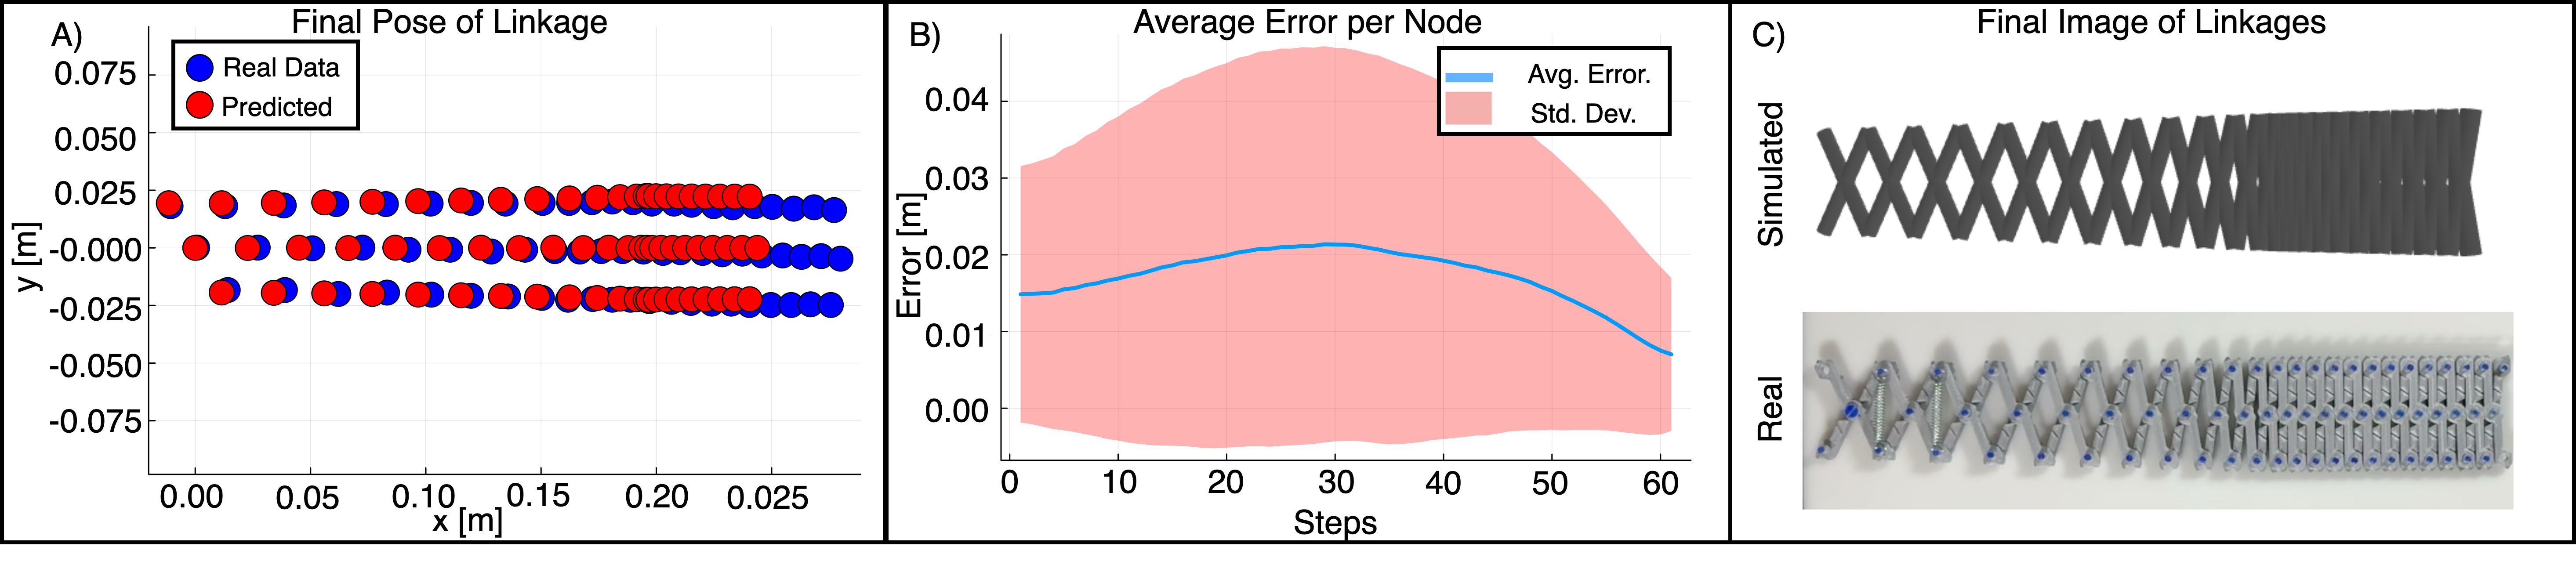
\includegraphics[width=\linewidth]{Figures/hardware_to_simulation_results.drawio.png}
    \caption{Comparison of real vs. simulated positions for the scissor mechanism. (A) The final pose of the linkage, showing real (red) and simulated (blue) positions of the scissor mechanism nodes. (B) Average error per node over time steps, with the blue line representing the mean error and the shaded red area indicating error variation. (C) Final images of the linkage: the top shows the simulated model, while the bottom displays the real-world scissor mechanism. This comparison qualitatively highlights the system’s ability to replicate real-world motion in simulation.}
    \label{fig:real_results}
\end{figure*}
\begin{figure}
    \centering
    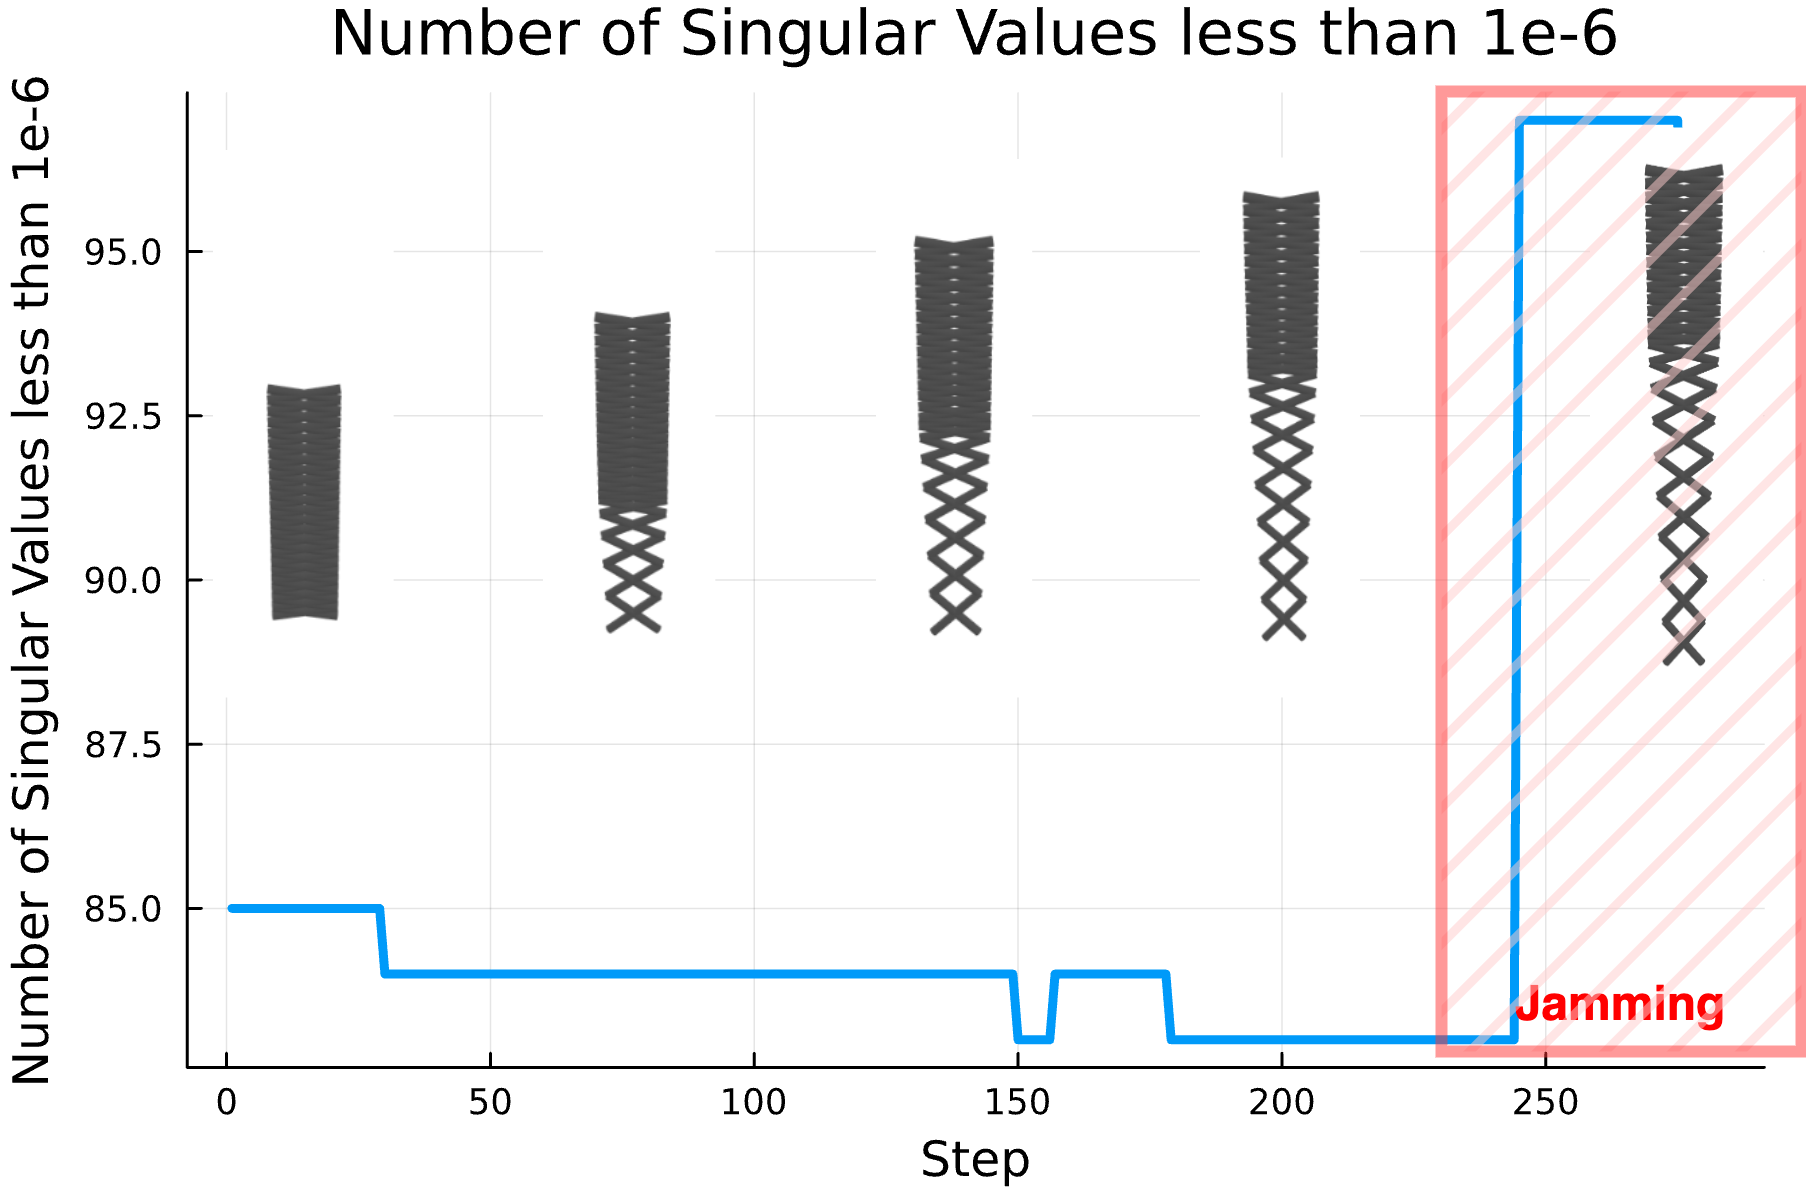
\includegraphics[width=0.6\linewidth]{Figures/Jamming_svds.drawio.png}
    \caption{Singular Value Decomposition (SVD) of the mechanism under loading conditions, showing the number of singular values less than 1e-6 over time steps. The increase in the number of small singular values indicates the onset of jamming (highlighted in the red-shaded region).}
    \label{fig:jamming-detection}
      \includegraphics[width=0.6\linewidth]{Figures/joint_reaction_forces.drawio.png}
    \caption{Visualization of joint constraint forces during jamming. The arrows represent joint reaction forces, with red indicating forces on the parent link and green showing forces on the child link. }
    \label{fig:constraint-force}
\end{figure}
% \begin{figure}
%     \centering
%     \includegraphics[width=\linewidth]{DOJO-CCK/Figures/joint_reaction_forces.drawio.png}
%     \caption{Visualization of joint constraint forces during jamming. The arrows represent joint reaction forces, with red indicating forces on the parent link and green showing forces on the child link. }
%     \label{fig:constraint-force}
% \end{figure}
\subsection{Hardware experiment results}
Initial experimentation was also performed on a 23-unit scissor mechanism. The mechanism is driven using two extension springs with a Spring force of 2870 N/m. The springs fail to deploy this linkage completely due to the joint clearance and friction. The positions of the joint locations are extracted using the OpenCV and co-tracker packages. We can assume a median error per node around 5 mm from the synthetic data experiment. The true values for the joint clearance are estimated by measuring using calipers to be around 0.4 mm. The true joint friction cannot be directly measured to provide a ground truth. The results for the hardware experiment can be seen in Figure \ref{fig:real_results}. We found that the best joint friction was around 0.003 Ns/m, and we fixed the joint clearance to a value of 0.4mm based on the true measurement. Figure \ref{fig:real_results}A shows the tracked locations from the real and simulated results. Figure \ref{fig:real_results}B shows the average error per node per time step, which is between 1-2 cm. This value is quite reasonable given that the resolution of the visual measurement is $\pm$5mm. Finally, Figure \ref{fig:real_results}C compares the simulated and real hardware qualitatively. This image shows that the joint limits on this simulated version do not match that of the real hardware, as the scissors are packing much tighter in the non-extended region. This could account for the position error between the simulated and real systems. These initial results are promising for future digital twin generation of linkage mechanisms and provide an interesting challenge for measurement resolution to capture joint tolerances. 
% TODO: Scissor Mechanism Position Tracking:
% % Present the real-world position tracking data from the slow-motion camera compared to the simulated positions from the digital twin.
% % Discuss any discrepancies between the simulated and real-world data, particularly in the context of joint clearance and friction.
% % Plot/Table: Real vs. simulated positions for the scissor mechanism.
% TODO: Bennett Linkage Position Tracking:
% % Show the real-world tracking data for the Bennett linkage using the motion capture system, compared to the simulation results.
% % Highlight how the digital twin captures the dynamics of the linkage and compare the joint clearance and friction estimations.
% % Plot/Table: Real vs. simulated positions for the Bennett linkage.

\subsection{Jamming Detection}
Finally, jamming and joint force analysis were explored using the above model. Jamming is a phenomenon in linkages that are frequently seen in hardware but under-explored in simulation modeling. This is likely due to the ill-conditioning that occurs when jamming takes place. Figure \ref{fig:jamming-detection} shows the number of singular values lower than 1e-6 over a 275-step deployment of the linkage. For most of the linkage deployment, the number of singular values stays around constant or decreases, likely due to numerical limitations. At step 250, the number of singular values sharply increases for several steps until the end of the simulation. This sharp increase in singular values means fewer degrees of freedom for the system to move in. The joint constraint forces are shown in Figure \ref{fig:constraint-force} with the forces acting on the child nodes of the constraint shown in green and the parent nodes in red. Further investigation on the significance of the magnitude and direction of the constraint forces is needed to better characterize why jamming occurs at this point in the deployment. 
% TODO: Jamming Detection Results
% Simulation Behavior Under Different Loading Conditions:
% Present the results from simulations with various loading conditions designed to induce jamming in both the scissor mechanism and Bennett linkage.
% Discuss the appearance of additional singular values in the SVD-based model reduction during jamming events.
% Show how the increase in thresholded singular values indicates a reduction in the degrees of freedom, correlating with the onset of jamming.
% Plot: Singular values under normal and jamming conditions
% Joint Constraint Forces During Jamming:
% Present the results of the simulation forces experienced by the joints during jamming events.
% Discuss how the digital twin captures the increase in constraint forces as the system jams, providing insights into mechanical limits.
% Figure: Visualization of joint constraint forces during jamming.





% TODO: TABLE Estimated Joint Clearance and Friction (Scissor Mechanism and Bennett Linkage)


